%%%%%%%%%%%%%%%%%%%%%%%%%%%%%%%%%%%%%%%%%%%%%%%%%%%%%%%%%%%%%%%%%
% Tese de Doutorado / Dept Fisica, CFM, UFSC                    %
% Andre@UFSC - 2014                                             %
%%%%%%%%%%%%%%%%%%%%%%%%%%%%%%%%%%%%%%%%%%%%%%%%%%%%%%%%%%%%%%%%%

%:::::::::::::::::::::::::::::::::::::::::::::::::::::::::::::::%
%                                                               %
%                          Capítulo 5                           %
%                                                               %
%:::::::::::::::::::::::::::::::::::::::::::::::::::::::::::::::%


\chapter{Caracterizando a PSF do CALIFA}
\label{sec:psf}

%***************************************************************%
%                                                               %
%                             PSF                               %
%                                                               %
%***************************************************************%
\section{Efeitos instrumentais e atmosféricos}
\label{sec:psf:teoria}

A PSF (sigla para {\em Point Spread Function}, em inglês) descreve a resposta de
um sistema de imageamento a uma fonte pontual. Observando uma fonte pontual no
infinito, que emite no comprimento de onda $\lambda$ com uma lente ideal de
diâmetro de abertura $D$, obtém-se uma imagem de diâmetro (em radianos) $\theta
\approx 1,22\frac{\lambda}{D}$. Esta imagem, conhecida como Disco de Airy, é a
figura de interferência causada por uma abertura circular, e limita a resolução
espacial teórica que se pode obter com um telescópio de uma dada abertura. Isto
vale para desde telescópios e câmeras pequenos, até telescópios espaciais.

Para um telescópio suficientemente grande, na superfície terrestre, a figura de
difração torna-se desprezível se comparada ao efeito causado pela turbulência
atmosférica, conhecida como {\em seeing}. Telescópios com diâmetro a partir de
$\sim\!20\,\mathrm{cm}$ já têm sua resolução espacial (no óptico) limitada pelo
{\em seeing}\footnote{Desconsiderando telescópios que aplicam técnicas de óptica
adaptativa, que não fazem parte do escopo deste trabalho.}. O modelo de
Kolmogorov, baseado em estudos de turbulência e desenvolvido por
\citet{Tatarskii1961}, descreve como as frentes de onda são perturbadas durante
a passagem por células de turbulência atmosférica. Uma excelente revisão sobre a
teoria da PSF é feita por \citet{Racine1996}. O perfil de Kolmogorov é dado pela
transformada de Bessel da função de transferência de modulação atmosférica dado
pelo modelo de Kolmogorov, e fica definido em função de uma integral sem forma
fechada, devendo ser resolvida numericamente. Costuma-se utilizar formas
funcionais que se aproximam do perfil de Kolmogorov. Gaussianas são usadas muito
frequentemente, mesmo não sendo adequadas. O perfil de \citet{Moffat1969} se
ajusta bem ao perfil de Kolmogorov numa faixa de $\sim\!7$ magnitudes em brilho
superficial, muito além do que a maioria dos casos de uso requer, e tem uma
forma bastante simples, dada por
\begin{equation*}
I(r) = \frac{I_0}{\left[1 + \left(\frac{r}{\alpha}\right)^2\right]^\beta},
\ \alpha = \frac{\mathrm{FWHM}}{2\sqrt{2^{1/\beta} - 1}}.
\end{equation*}
Dois parâmetros controlam a forma da PSF neste perfil: a largura a meia altura
($\mathrm{FWHM}$) e o índice $\beta$, que controla a intensidade das ``asas'' da
PSF. Com $\beta\!\to\!\infty$, o perfil de Moffat torna-se uma gaussiana. O
melhor ajuste ao perfil de Kolmogorov se obtém quando $\beta\!=\!4$ (Figura
\ref{fig:PSFRacine}).

\begin{figure}
	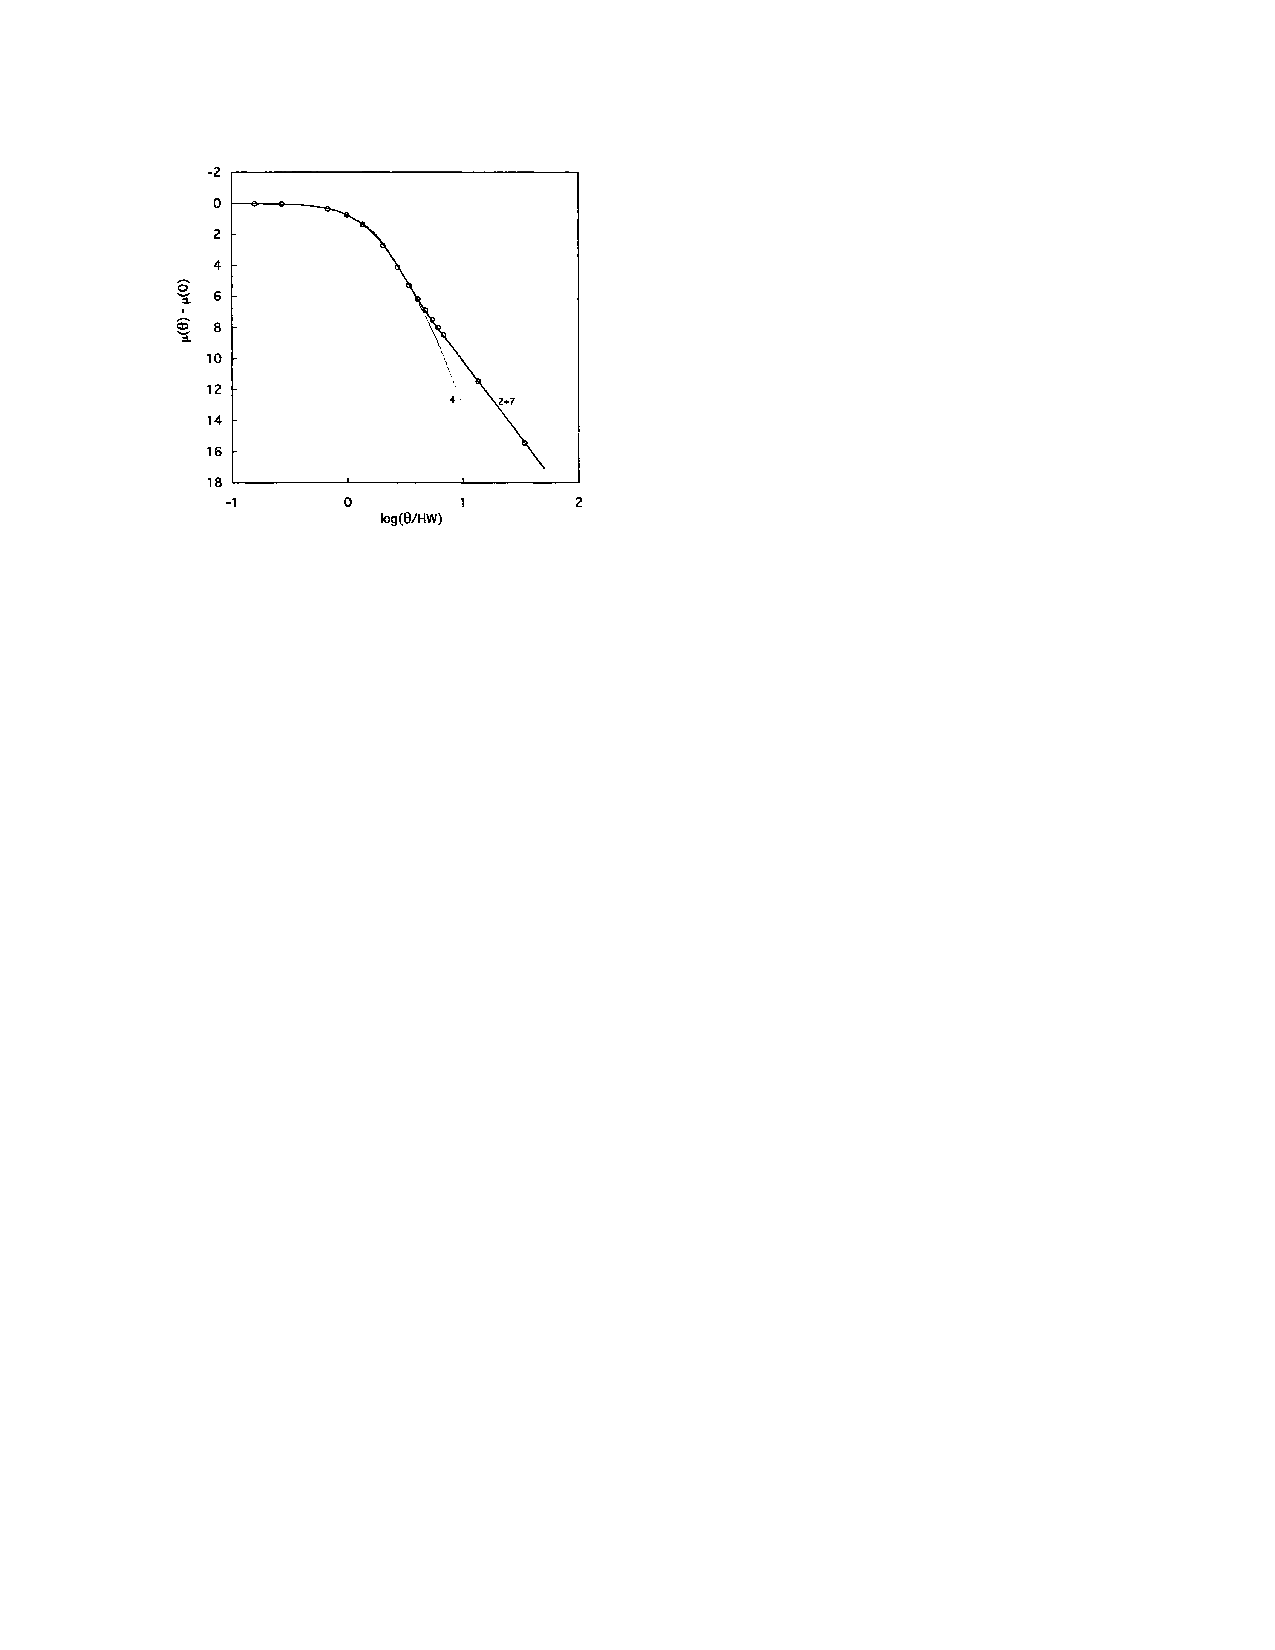
\includegraphics{figuras/PSFRacine}
	\caption[Ajuste de perfil de Moffat ao modelo de PSF de Kolmogorov.]
	{Ajuste de perfil de Moffat (linhas sólidas) ao modelo de PSF de Kolmogorov
	(círculos abertos). A linha fina, é um perfil de Moffat com $\beta\!=\!4$, e a
	linha espessa é a soma de dois perfis de Moffat, com $\beta\!=\!7$ ($80\,\%$
	do fluxo) e $\beta\!=\!2$ ($20\,\%$ do fluxo). Retirado de \citet{Racine1996}.}
	\label{fig:PSFRacine}
\end{figure}

Se a PSF é constante em todo o campo, seu efeito na imagem pode ser calculado
como a convolução entre a imagem da PSF e a imagem original. Isto tem um custo
computacional extremamente elevado, especialmente quando se utiliza algum
procedimento iterativo como um ajuste de modelo. Uma convolução, em cálculo
numérico, significa calcular uma integral em duas dimensões para cada {\em
pixel}, ou seja, escala com $\mathcal{O}(n^2)$. Um truque bastante comum é
utilizar transformadas de Fourier para simplificar este cálculo e transformá-lo
num algoritmo que escala com $\mathcal{O}(n \log n)$. Se $I$ é a imagem original
e $I^\mathrm{PSF}$ a imagem da PSF, a imagem final $I^\ast$ é dada por
\begin{equation*}
I^\ast = I \otimes I^\mathrm{PSF}.
\end{equation*}
Aplicando a transformada de Fourier,
\begin{equation*}
\mathcal{F}\{I^\ast\} &= \mathcal{F}\{I \otimes
I^\mathrm{PSF}\} \\
&= \mathcal{F}\{I\} \cdot \mathcal{F}\{I^\mathrm{PSF}\},
\end{equation*}
ou seja, troca-se uma convolução por uma multiplicação. Para obter a imagem
final, basta aplicar a transformada de Fourier inversa sobre o produto. A
transformada de Fourier da PSF é sempre a mesma, logo a cada iteração apenas
duas integrais numéricas em duas dimensões são necessárias: a transformada da
imagem original e a transformada inversa para a imagem final. O ganho é tão
significativo que praticamente todos os programas de ajuste de imagens
astronômicas utilizam transformadas de Fourier para convoluir a imagem.


%***************************************************************%
%                                                               %
%                       PSF do CALIFA                           %
%                                                               %
%***************************************************************%
\section{Medindo a PSF}

Para determinar as caraterísticas da PSF, idealmente é preciso observar um
objeto pontual brilhante, em várias regiões do campo do detector, e com as
mesmas condições atmosféricas que as observações. Raramente estas condições são
preenchidas, mesmo para fotometria CCD com campos muito grandes. Assim, conhecer
a PSF em instrumentos IFU não é uma tarefa trivial. Ainda há o fato de que as
imagens são reconstruídas através de técnicas de {\em dithering} (ver Seção
\ref{sec:ifs:instrumentacao}), e dependendo o algoritmo utilizado, a PSF pode
nem sequer ser analítica. Entretanto, é preciso de algum modo obter uma
aproximação da forma da PSF para poder modelar a morfologia de uma galáxia
(Capítulo \ref{sec:morph}), especialmente o seu bojo. O procedimento descrito a
seguir é mais um esforço para entender a PSF e poder realizar a decomposição
morfológica do que um estudo aprofundado sobre o tema.

Para o CALIFA, observar campos estelares para caracterizar a PSF significaria a
redução no número de galáxias na amostra final do {\em survey}. Dadas as
restrições de tempo de telescópio e de significância estatística da amostra,
além do fato de a PSF não ser fundamental para os casos científicos alvo do {\em
survey}, estas observações não foram realizadas. Porém, sendo um {\em survey}
espectroscópico, o CALIFA necessita de observações de ``velas padrão'' para
calibrar o fluxo das galáxias. Foram observadas 45 estrelas para este fim.
Estas estrelas foram obsevadas no centro no campo de observação do instrumento,
com um tempo de exposição muito menor do que o das galáxias ($120\,\mathrm{s}$
contra $900\,\mathrm{s}$). Esta amostra foi denominada ``estrelas de
calibração''. Alternativamente, pode-se procurar estrelas que apareçam na frente
das galáxias do {\em survey}. Neste caso a vantagem é que as estrelas têm o
mesmo tempo de exposição das galáxias, e são observadas nas mesmas condições
atmosféricas. Porém, não se encontra estas estrelas intrometidas em todos os
cubos, logo obter uma PSF para cada um deles está descartado. Outro problema em
potencial é que elas em geral, por construção do {\em survey}, são fracas e se
localizam na periferia do campo de observação. Esta amostra foi denominada
``estrelas de campo'', com 9 estrelas suficientemente brilhantes escolhidas em
cubos de galáxias {\em early type}. As duas amostras de estrelas reaproveitadas
foram usadas para caracterizar a PSF do CALIFA com o procedimento descrito a
seguir.

\begin{figure}
	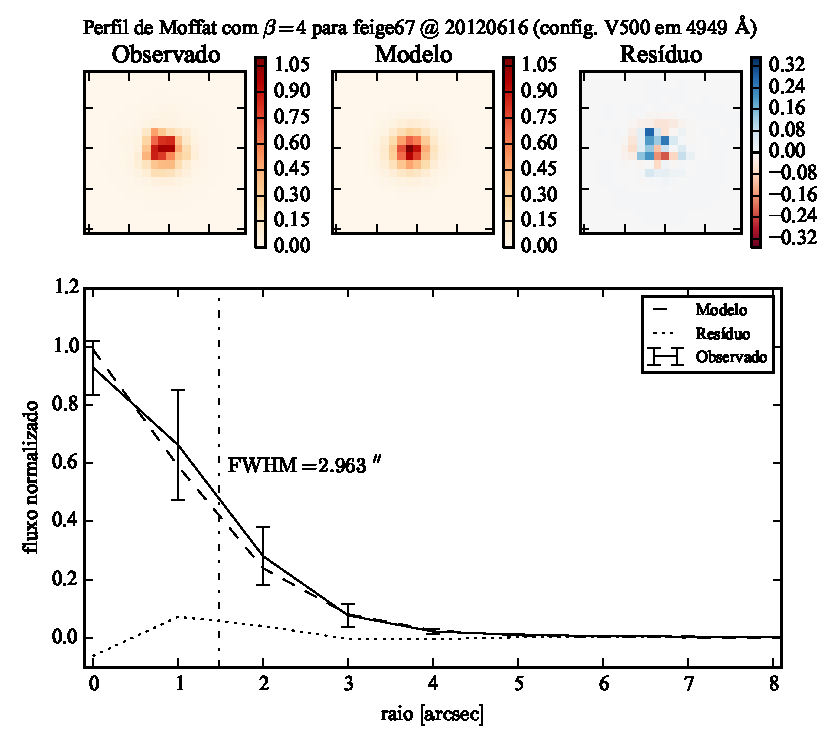
\includegraphics{figuras/PSFMoffatBeta4_exemplo}
	\caption[Exemplo de ajuste de PSF para estrela de calibração.]
	{Exemplo de ajuste de PSF para a estrela de calibração Feige67, observada em
	16/06/2012, com a cofiguração V500. O modelo ajustado foi um perfil de
	Moffat elipsoidal com $\beta=4$. Nos painéis superiores estão imagens do fluxo
	observado numa caixa de $400\,\angstrom$ centrada em $4949\,\angstrom$,
	do modelo ajustado e do resíduo do ajuste. No painel inferior mostra-se o
	perfil de brilho radial médio: observado (linha sólida, onde as barras de erro
	são $1\,\sigma$ da média), modelo (linha tracejada, e a linha traço-ponto marca
	a largura a meia altura $\mathrm{FWHM}=2,963\,\arcs$) e resíduo (linha
	pontilhada).}
	\label{fig:PSFExemplo}
\end{figure}

O modelo utilizado foi um perfil de Moffat 2-d elipsoidal, com $\beta\!=\!4$,
conforme visto na Seção \ref{sec:psf:teoria}. Os cubos foram combinados em
caixas de $400\,\angstrom$ de largura, gerando 10 imagens de fluxo e incerteza
para cada estrela. Estas imagens foram ajustadas aos modelos através de um
programa desenvolvido utilizando a biblioteca PYTHON-IMFIT\footnote{PYTHON-IMFIT
é uma biblioteca baseada no programa IMFIT de \citet{Erwin2015}, a mesma
utilizada no programa de decomposição morfológica, ver Seção
\ref{sec:morph:comp:depLambda}.}. O resultado do ajuste são os parâmetros do
perfil de Moffat e a estatística $\chi^2$ do melhor modelo. A Figura
\ref{fig:PSFExemplo} ilustra o ajuste feito para uma estrela de calibração, numa
faixa espectral próxima a $5000\,\angstrom$.

\begin{figure}
	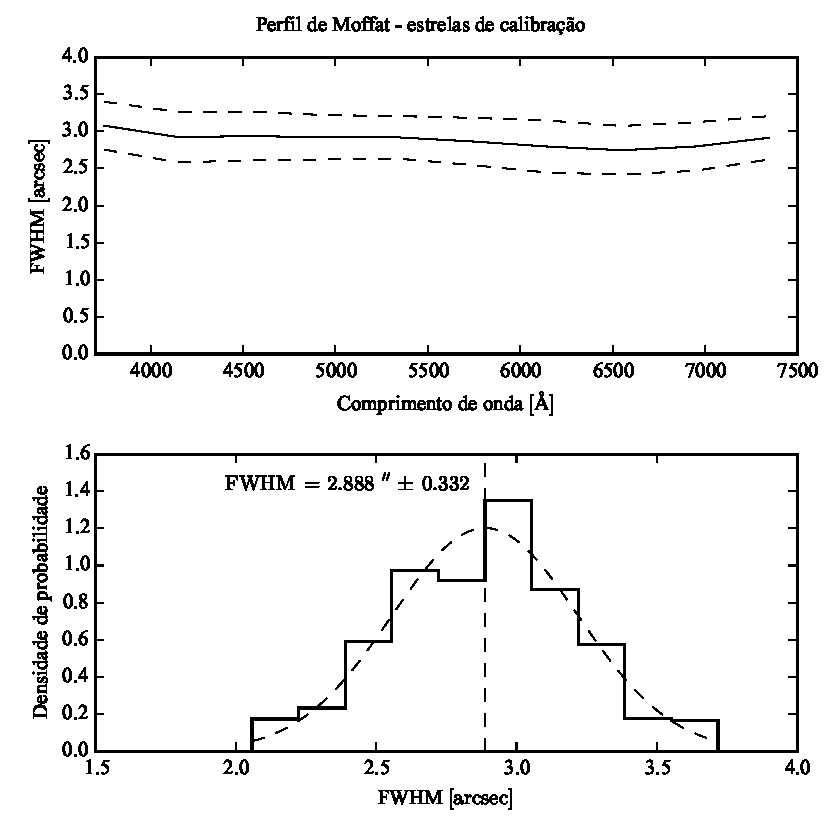
\includegraphics{figuras/PSFMoffatBeta4_calib}
	\caption[PSF do CALIFA -- estrelas de calibração.]
	{PSF do CALIFA modelada como um perfil de Moffat com $\beta=4$, utilizando 45
	estrelas de calibração. {\em Acima}: FWHM da PSF em função do comprimento de
	onda (caixas de $400\,\angstrom$). As linhas tracejadas indicam a distribuição
	em $1\ \sigma$. {\em Abaixo}: Histograma da FWHM da PSF, ponderado pela
	verossimilhança do modelo em todos os comprimento de onda de todas as estrelas,
	com $\mathrm{FWHM}=2,888 \pm 0,332\,\arcs$.}
	\label{fig:PSFCalib}
\end{figure}

Este procedimento foi realizado para as 45 estrelas de calibração, e o resultado
pode ser visto na Figura \ref{fig:PSFCalib}. Praticamente não há dependência da
PSF com o comprimento de onda, como se pode verificar no painel superior da
figura. Na mesma figura, no painel inferior, mostra-se um histograma ponderado
pela verossimilhança ($\operatorname{e}^{-\chi^2/2}$) de todos os ajustes (todas
as estrelas em todas as caixas de comprimento de onda). Desta distribuição
obtém-se uma largura a meia altura média de $\mathrm{FWHM} = 2,888 \pm
0,332\,\arcs$. A elipticidade ($\epsilon = 1 - b/a$) média encontrada é de
$\epsilon = 0,097 \pm 0,065$, ou seja, a PSF é praticamente circular. A
incerteza nos dois casos representa o desvio padrão ($1\,\sigma$) da média
ponderada. O mesmo vale para todas as incertezas obtidas no resto desta seção.

\begin{figure}
	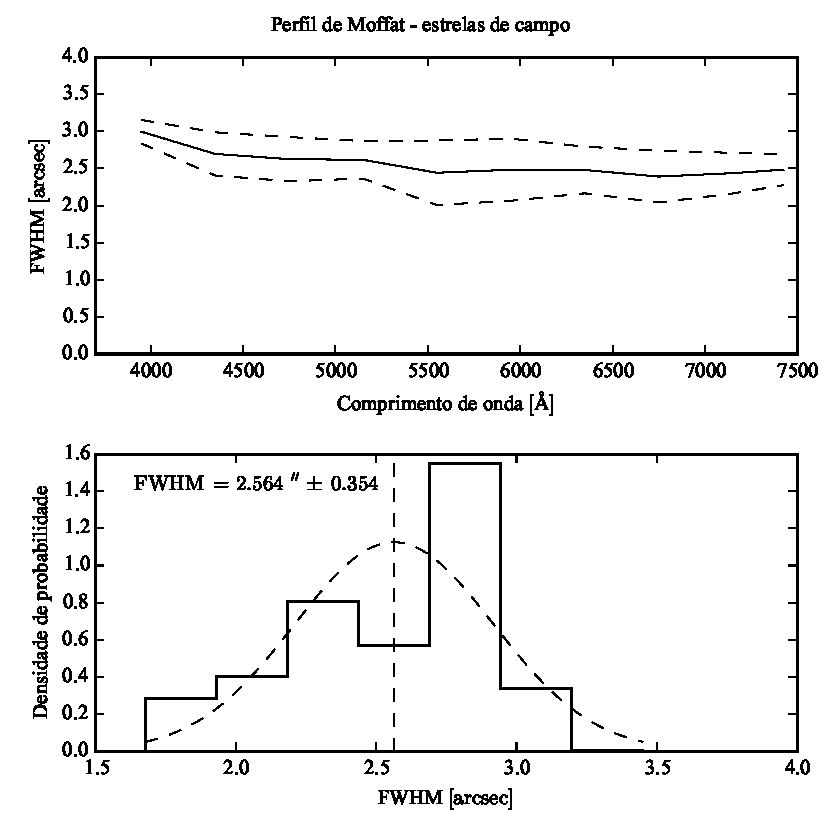
\includegraphics{figuras/PSFMoffatBeta4_field}
	\caption[PSF do CALIFA -- estrelas de campo.]
	{PSF do CALIFA modelada como um perfil de Moffat com $\beta=4$, utilizando 9
	estrelas de campo, na frente das galáxias observadas. {\em Acima}: FWHM da PSF
	em função do comprimento de onda (caixas de $400\,\angstrom$). As linhas
	tracejadas indicam a distribuição em $1\ \sigma$. {\em Abaixo}: Histograma da
	FWHM da PSF, ponderada pela verossimilhança do modelo em todos os comprimentos
	de onda de todas as estrelas, com $\mathrm{FWHM}=2,564 \pm 0,354\,\arcs$.}
	\label{fig:PSFField}
\end{figure}

O mesmo procedimento foi realizado para as 9 estrelas de campo, presentes nos
cubos de galáxias do {\em survey} e normalmente mascarados por não serem de
interesse no estudo do espectro das galáxias. As estrelas desta amostra estão na
frente de galáxias com simetria axial (elípticas e S0). Dado um cubo de uma
galáxia, recortou-se 7 {\em spaxels} ao redor da estrela, gerando dois cubos: um
da galáxia, com a estrela mascarada, e outro da estrela. Neste ponto o cubo da
estrela ainda está contaminado pela luz da galáxia. Então, considerando que a
galáxia tem simetria axial, calculou-se um perfil de brilho radial médio da
galáxia (ver Seção \ref{sec:pycasso:Pycasso}, Figura \ref{fig:radprofIdade}),
para cada comprimento de onda. Com este perfil, é possível estimar quanto a
galáxia está contribuindo para a luz de cada {\em spaxel} do cubo da estrela,
pois a distância de cada {\em spaxel} ao centro da galáxia é conhecido. Criou-se
assim um cubo de ``luz de fundo'' para a mesma região que contém a estrela.
Subtraindo o cubo de fundo do cubo da estrela, obteve-se um cubo com apenas a
luz proveniente da estrela. Este cubo foi então analisado da mesma forma que os
cubos de estrelas de calibração, com os resultados mostrados na Figura
\ref{fig:PSFField}. Da mesma forma, não há dependência da FWHM da PSF com o
comprimento de onda, com $\mathrm{FWHM}=2,564 \pm 0,354\,\arcs$ e elipticidade
$\epsilon=0,093 \pm 0,059$.

Há uma diferença considerável no valor obtido para a FWHM da PSF nos dois casos,
embora eles estejam a cerca de $1\,\sigma$ de separação. Isto poderia indicar
uma diferença sistemática entre a PSF das estrelas de calibração e a PSF das
estrelas de campo. Todavia, observando atentamente o histograma de FWHM das
estrelas de campo (painel inferior da Figura \ref{fig:PSFField}), pode-se notar
que a distribuição possui um excesso próximo a $2,8\,\arcs$. Isso parece indicar
que a FWHM da PSF das estrelas de campo é em geral maior do que o estimado pela
média ponderada, já que a distribuição se desvia de uma gaussiana. Isto, aliado
ao fato de que o tamanho da amostra de estrelas de calibração (45) é maior do
que o das estrelas de campo (9), fez com que se escolhesse a medida da primeira
amostra como a mais confiável.

Já com os valores de elipticidade ($\epsilon$) obtidos nos dois casos, os
semieixos maior e menor da FWHM estão dentro da faixa de $1\,\sigma$ um do
outro. E em ambos os casos, $\epsilon$ é muito próximo a zero, dentro da
incerteza. Levar a elipticidade em conta seria adicionar uma complexidade
desnecessária (e possivelmente artificial) ao modelo de PSF.

Assim, a PSF adotada neste trabalho é um perfil de Moffat com simetria axial,
$\beta\!=\!4$ e $\mathrm{FWHM}=2,9 \pm 0,3\,\arcs$. Este foi o mesmo
procedimento para fazer a caracterização da PSF publicada no DR2 do CALIFA
\citep{GarciaBenito2015}, mas com uma diferença. Naquele caso, modelou-se tanto
FWHM quanto $\beta$, obtendo-se $\mathrm{FWHM}=2,39 \pm 0,26\,\arcs$ e
$\beta=1,73 \pm 0,11$. A diferença está basicamente em qual região da PSF se
está interessado. Por uma questão geométrica, há mais {\em pixels} longe do
centro do perfil, o que acaba causando mais peso destas regiões periféricas no
modelo escolhido pelo ajuste (ver as barras de erro cada vez menores com a
distância, na Figura \ref{fig:PSFExemplo}, que são a grosso modo inversamente
proporcionais ao peso). Porém, na maioria destes {\em pixels} periféricos o
fluxo proveniente da estrela já está submerso no ruído, achatando o perfil (isto
é, diminuindo $\beta$). O ajuste resultante é então pior nas regiões centrais,
com peso menor.
No caso do ajuste morfológico de uma galáxia, isto pode causar problemas na
determinação dos parâmetros do bojo. Assim, optou-se por refazer a análise ds
PSF para esta tese com $\beta$ fixo.

% End of this chapter
